% Copyright 2021 Edoardo Riggio

% Licensed under the Apache License, Version 2.0 (the "License");
% you may not use this file except in compliance with the License.
% You may obtain a copy of the License at

% 	http://www.apache.org/licenses/LICENSE-2.0

% Unless required by applicable law or agreed to in writing, software
% distributed under the License is distributed on an "AS IS" BASIS,
% WITHOUT WARRANTIES OR CONDITIONS OF ANY KIND, either express or implied.
% See the License for the specific language governing permissions and
% limitations under the License.

\documentclass{article}

\usepackage{hyperref, amsmath, graphicx}
\usepackage{fancyvrb,newverbs,xcolor}

\definecolor{cverbbg}{gray}{0.93}

\newenvironment{cverbatim}
 {\SaveVerbatim{cverb}}
 {\endSaveVerbatim
  \flushleft\fboxrule=0pt\fboxsep=.5em
  \colorbox{cverbbg}{\BUseVerbatim{cverb}}%
  \endflushleft
}

\newenvironment{lcverbatim}
 {\SaveVerbatim{cverb}}
 {\endSaveVerbatim
  \flushleft\fboxrule=0pt\fboxsep=.5em
  \colorbox{cverbbg}{%
    \makebox[\dimexpr\linewidth-2\fboxsep][l]{\BUseVerbatim{cverb}}%
  }
  \endflushleft
}

\newcommand{\ctexttt}[1]{\colorbox{cverbbg}{\texttt{#1}}}
\newverbcommand{\cverb}
  {\setbox\verbbox\hbox\bgroup}
  {\egroup\colorbox{cverbbg}{\box\verbbox}}

\begin{document}
\begin{titlepage}
    \begin{center}
        \vspace*{1cm}
        
        \Huge
        \textbf{Operating Systems Cheatsheet}
        
        \vspace{0.5cm}
        \LARGE
        
        \vspace{.5cm}
        
        Edoardo Riggio
   		  \vspace{1.5cm}
       
        \vfill
        
        \today
        
        \vspace{.8cm}
          \Large
          Operating Systems - SP. 2021 \\
        Computer Science\\
        Universit\`{a} della Svizzera Italiana, Lugano\\
        
    \end{center}
\end{titlepage}

\tableofcontents

\newpage

\section{Introduction}
\subsection{Computer System}
A \textbf{computer system} can be roughly divided into four parts:

\begin{itemize}
	\item \textbf{Hardware}
	\vspace{.2cm} \\
	It provides the basic computing resources for the system, such as CPU, memory and I/O devices.
	
	\item \textbf{Operating System}
	\vspace{.2cm} \\
	It controls and coordinates the use of hardware among various applications and users.
	
	\item \textbf{Application Programs}
	\vspace{.2cm} \\
	They define the ways in which the resources are used to solve users' computing problems.
	
	\item \textbf{User}
	\vspace{.2cm} \\
	They are people, machines and other computers.
\end{itemize}

\subsection{Operating System}
An \textbf{operating system} is a program that manages a computer's hardware. It also acts as an intermediary between the computer user and the computer hardware. The main goals of an OS are for example:

\begin{itemize}
	\item Execute user programs
	\item Make the system convenient to use
	\item Efficiently use the computer hardware
\end{itemize}
The operating system provides the environment within which other programs can do useful work. An OS is mainly two things:

\begin{itemize}
	\item \textbf{Resource Allocator}
	\vspace{.2cm} \\
	The operating system manages the resources offered by the computer hardware -- such as CPU time, memory space, file-storage space, I/O devices... It must also decide how to allocate these resources so that it can operate the computer efficiently and fairly.
	
	\item \textbf{Control Program}
	\vspace{.2cm} \\
	The operating system manages the execution of user programs to prevent errors and improper use of the computer.
\end{itemize}
There is no universal definition for an operating system. It exists because it offers a reasonable way to solve the problem of creating a usable computer system. \\ \\
There is also no accepted definition of what is part of the operating system. A good approximation could be "everything that a vendor includes and ships when a user orders an operating system". \\ \\
A possible way of defining an operating system is that this is the one program running at all times on the computer -- also known as the \textbf{kernel}. Everything that is not the kernel can be either:

\begin{itemize}
	\item \textbf{System Program}
	\vspace{.2cm} \\
	They are programs associated with the operating system but not part of the kernel.
	
	\item \textbf{Application Programs}
	\vspace{.2cm} \\
	They are the programs that are not associated with the operation of a system.
\end{itemize}

\subsection{Computer System Organisation}
Modern computers consist of 1 or more CPUs and a number of device controllers connected through a common bus that provides access to shared memory. \\ \\
In order for a computer to start running, it needs an initial program to run. Such program is called \textbf{bootstrap program}. This initializes all aspects of an operating system. This program tends to be simple, and is typically stored in ROM (Read-Only Memory) or in EEPROM (Electrically Erasable Programmable Read-Only Memory).\\ \\
When the kernel is loaded and executing, it starts providing services to the system and its users. Some services, though, are provided outside of the kernel, by system programs that are loaded into memory at boot time. Such programs are called \textbf{system daemons} and are those that run the entire time that the kernel is running.\\ \\
In an operating system, the occurrence of events are usually signaled by an \textbf{interrupt} either from the hardware or the software. Hardware may trigger interrupts by sending a signal to the CPU, while software may trigger interrupts by executing a \textbf{system call}. When the CPU is interrupted, it stops what it's doing and immediately transfers execution to a fixed location. Since interrupts must be handled quickly, a table of pointers to interrupt routines can be used in order to provide the necessary speed. Such table is called an \textbf{interrupt vector}, and is stored in the first hundred or so locations in low memory.

\subsection{Storage Structure}
The CPU can load instructions only from memory, so any program to run must be stored there. Computers run most of their programs from re-writable main memory such as RAM (Random Access Memory) or DRAM (Dynamic Random Access Memory) -- which is used as main memory. Static programs are instead stored in ROM or EEPROM. There are problems with main memory, two of which being:

\begin{itemize}
	\item It is usually too small to store all programs and data permanently
	\item It is \textbf{volatile}, meaning that it looses everything when powered off
\end{itemize}
These are the main reasons to why most systems also provide secondary storage as an extension of main memory. This type of storage is capable to hold large quantities of data permanently.

\subsection{I/O Structure}
Operating systems typically have a device driver for each device controller. A \textbf{device controller} is in charge of a specific type of device. Instead, \textbf{device drivers} provide the rest of the operating system with a uniform interface to the device. \\ \\
In order to start an I/O operation, the device driver loads the appropriate registers within the device controller. The controller then starts the transfer of data from the device to its local buffer. Once the transfer is complete, the controller sends an interrupt to the driver. \\ \\
When dealing with the transfer of large amounts of data, the previous solution generates a lot of overhead. In order to reduce that, \textbf{DMA} (Direct Memory Access) is used. After setting everything up, the device controller transfers an entire block of data to/from its buffer from/to memory directly -- with no intervention from the CPU. Only one interrupt is generated for block.

\subsection{Multiprocessor Systems}
\textbf{Multiprocessor systems} have two or more processors in close communication, sharing the computer bus, and sometimes the clock, memory and peripheral devices. These systems have three main advantages:

\begin{itemize}
	\item \textbf{Increased Throughput}
	\vspace{.2cm} \\
	The more processors, the more speed. However, the more processors we add, the more overhead there is in order to maintain all the parts working correctly.
	
	\item \textbf{Economy of Scale}
	\vspace{.2cm} \\
	Multiprocessor systems cost less than multiple single-processor systems. All resources are shared in the first system.
	
	\item \textbf{Increased Reliability}
	\vspace{.2cm} \\
	The failure of one processor will not halt the system, just slow it down. The ability to continue providing service proportional to the level of surviving hardware is called \textbf{graceful degradation}. Systems that go beyond graceful degradation are called \textbf{fault tolerant}, because they can suffer a failure of any single component and still be able to work.
\end{itemize}
The multiple-processor systems in use today use two main systems:

\begin{itemize}
	\item \textbf{Asymmetric Multiprocessing}
	\vspace{.2cm} \\
	Here, to each processor is assigned a specific task. A boss processor controls the system by allocating work to the worker processes.
	
	\item \textbf{Symmetric Multiprocessing}
	\vspace{.2cm} \\
	Each processor performs all tasks within the operating system. All processors are peers.
\end{itemize}

\subsection{Multicore Systems}
A system is \textbf{multicore} when it includes multiple cores on a single chip. This CPU design can be more efficient than single-core CPU designs. These advantages are:

\begin{itemize}
	\item \textbf{Speed}
	\vspace{.2cm} \\
	On-chip communication is faster than between-chip communication.
	
	\item \textbf{Power Consumption}
	\vspace{.2cm} \\
	Multicore CPUs consume a considerably less amount of energy than multiple single-core CPUs.
\end{itemize}
In multicore CPU designs, each core has its own register set as well as its own local cache. \\ \\
Some operating systems have the ability to continue providing service proportional to the level of surviving hardware. This is known as \textbf{graceful degradation}. Other systems go beyond graceful degradation, this is known as a \textbf{fault tolerant} system. These systems can suffer a failure of any single component and still continue operation. \\ \\
Multiple-processor systems in use today are of two types:

\begin{itemize}
	\item \textbf{Asymmetric Multiprocessing}
	\vspace{.2cm} \\
	Each processor is assigned to a specific task, and a poss processor controls the system. This scheme defines a boss-worker relationship.
	
	\item \textbf{Symmetric Multiprocessing}
	\vspace{.2cm} \\
	Each processor performs all tasks within the operating system. Here, all processors are peers.
\end{itemize}

\subsection{Operating System Structure}
One of the most important aspects of operating systems is the ability to \textbf{multiprogram}. Multiprogramming increases CPU utilization by organizing jobs so that the CPU always has one to execute. The operating system keeps several jobs in memory simultaneously. Jobs are initially kept on the disk in the \textbf{job pool}. This pool consists of all processes residing on the disk awaiting for allocation of main memory. \\ \\ \textbf{Multitasking} is a logical extension of multiprogramming. In time-sharing systems, the CPU executes multiple jobs by switching among them. Switching occurs so frequently that users can interact with each program while it's running. A time-shared machine allows multiple users to share the computer simultaneously. This type of machine uses CPU scheduling and multiprogramming in order to provide each user with a part of the computer. Each user has at least one separate program in memory. Such programs are called \textbf{processes}. \\ \\
If several jobs are brought into memory, and there is not enough room for them, \textbf{job scheduling} is used in order to make the decision of choosing. If several jobs are ready to run at the same time, \textbf{CPU scheduling} is used in order to make the decision of which job to run first. \\ \\
A method used in order to ensure reasonable response times is \textbf{virtual memory}. This technique allows for the execution of a process that is not completely in memory. The main advantage of virtual memory is that it enables users to run processes that are larger than actual physical memory.

\subsection{Operating-Systems Operations}
Modern operating systems are \textbf{interrupt driven}. Events are almost always signaled by the occurrence of either an interrupt or a trap. A \textbf{trap} is a software-generated interrupt caused by either an error or by a request from a user program. Operating systems also need to make sure that an interrupt or trap that happens for one user is propagated and affect other users as well.

\subsubsection{Dual Mode Operation}
In order to ensure the proper execution of the OS, we must be able to distinguish between user defined and OS code. In order to do this we need at lest two modes of operation:

\begin{itemize}
	\item \textbf{Kernel Mode}
	\item \textbf{User Mode}
\end{itemize}
A bit, called the \textbf{mode bit}, is used by the operating system to indicate the current mode of execution (0 = kernel mode, 1 = user mode). By switching this bit we can know if code is running in kernel mode or in user mode. \\ \\
When a user program tries to run privileged commands, a trap occurs in which the operating system evaluates the command. If it is accepted, then the mode bit switches to 0 and the command is executed in kernel mode. After which the mode bit is set again to 1. 

\subsubsection{Timer}
A \textbf{timer} can be set in order to interrupt the computer after a specific period of time. This period may be fixed or variable. If the counter reaches 0, an interrupt occurs and the control transfers directly to the operating system.

\subsection{Process Management}
A \textbf{process} is an active entity that uses resources of a system. This is the unit of work in a system. A system consists of a collection of processes, both OS and user processes. The operating system is responsible for the following:

\begin{itemize}
	\item Scheduling processes and threads of a CPU
	\item Crating and deleting both user and system processes
	\item Suspending and resuming processes
	\item Providing mechanisms for process synchronization
	\item Providing mechanisms for process communication
\end{itemize}

\subsection{Memory Management}
To improve both the utilization of CPU and the responsiveness of the computer, they must keep several programs in memory, creating a need for memory management. The OS is responsible for the following:

\begin{itemize}
	\item Keeping track of which parts of memory are currently being used and who is using them
	\item Deciding which processes and data needs to be moved in and out of memory
	\item Allocating and deallocating memory as needed
\end{itemize}

\subsection{Storage Management}
In order to make the computer system convenient for users, the OS provides a uniform, logical view of information storage. The operating system abstracts from the physical properties of its storage devices to define a logical storage unit, the \textbf{file}. The operating system maps files onto physical media and accesses these files via the storage devices. \\ \\
These files generally represent programs or data. furthermore, files are organized into directories in order to make them easier to use, The OS is responsible for the following:

\begin{itemize}
	\item Creating and deleting files
	\item Creating and deleting directories to organize files
	\item Supporting primitives for manipulating files and directories
	\item Mapping files onto secondary storage
	\item Backing up files on stable, nonvolatile storage media
	\item Free-space management
	\item Storage allocation
	\item Disk scheduling
\end{itemize}

\subsection{Caching}
\textbf{Caching} is an important principle of computer systems. Information is normally stored in some storage system. As it is used, it is copied in the cache on a temporary basis. Since cache is very fast, it is the first place the computer goes when searching for information. If said information is not found in cache, it is looked for in main memory, then secondary memory and so on. \\ \\
Caches have limited sizes, so \textbf{cache management} is used in order to make caches efficient. \textbf{Cache coherency} is used to make sure that an updated copy of some data is always the same in local caches. This is true when we are in a multiprocessor environment where each of the CPUs also contain local caches.

\subsection{I/O Systems}
The I/O subsystem hides from the user the peculiarities of specific hardware devices. It consists of several components:

\begin{itemize}
	\item A memory-management component that includes buffering, caching and spooling
	\item A general device-driver interface
	\item Drivers for specific hardware devices
\end{itemize}
Only the drivers know the peculiarities of the specific device to which it is assigned.

\subsection{Protection and Security}
If a computer system has multiple users and allows concurrent execution of processes, then access to data must be regulated. An unprotected resource cannot defend against use or misuse by users.

\section{System Structures}
\subsection{Operating System Services}
An operating system provides a set of services, such as:

\begin{itemize}
	\item \textbf{User Interface}
	\vspace{.2cm} \\
	The \textbf{UI} (User Interface), can take several forms, such as \textbf{GUI} (Graphical User Interface) or \textbf{CLI} (Command-Line Interface). It offers a way for the user to easily interact with the machine.
	
	\item \textbf{Program Execution}
	\vspace{.2cm} \\
	The system must be able to load programs into memory and run them. The programs must also be able to end their execution either normally or by throwing an exception.
	
	\item \textbf{I/O Operations}
	\vspace{.2cm} \\
	The operating system must provide the means for the user to be able to interact with I/O, since users cannot control it directly.
	
	\item \textbf{File-System Manipulation}
	\vspace{.2cm} \\
	The ability of being able to delete, create or modify files and directories. The operating system also offers a way to set permissions to files and directories such that only authorized users can access them.
	
	\item \textbf{Communications}
	\vspace{.2cm} \\
	Enabling processes to be able to exchange messages between each other. Communication may be implemented either by shared memory or by message passing.
	
	\item \textbf{Error Detection}
	\vspace{.2cm} \\
	The operating system needs to properly detect and correct errors constantly.
\end{itemize}
Another set of services in place to ensure the efficient operation of a system is:

\begin{itemize}
	\item \textbf{Resource Allocation}
	\vspace{.2cm} \\
	Resources need to be allocated whenever there are multiple users or multiple jobs running at the same time.
	
	\item \textbf{Accounting}
	\vspace{.2cm} \\
	The operating system needs to keep track of which users use how much and what kind of computer resources.
	
	\item \textbf{Protection and Security}
	\vspace{.2cm} \\
	When several separate processes execute concurrently, it should not be possible for one process to interfere with the others or with the operating system itself. Also authentication is a form of security. In this way non-authorized users cannot access sensitive data.
\end{itemize}

\subsection{Command Interpreters}
There are two main ways to interact with computer systems:

\begin{itemize}
	\item \textbf{Command Interpreters}
	\vspace{.2cm} \\
	Interpreters are known as \textbf{shells}, and can be multiple on a single machine. The main function of these shells is to get and execute the next user-specified command.
	
	\item \textbf{Graphical User Interfaces}
	\vspace{.2cm} \\
	The GUI first appeared on the Xerox Alto in 1973. Mac OSX adopted the Aqua themed GUI, while Microsoft MSOS. KDE and Gnome are instead used in Linux an UNIX systems.
\end{itemize}

\subsection{System Calls}
\textbf{System calls} provide an interface to the services made available by the operating system. They are typically written in either C or C++ -- even though assembly code might be needed for directly accessing hardware. \\ \\
The \textbf{API} (Application Programming Interface) specifies a set of functions that are available to an application programmer, including parameters and return values. Some APIs available to programmers are:

\begin{itemize}
	\item Windows API
	\item POSIX API
	\item Java API
\end{itemize}
The \textbf{system-call interface} intercepts function calls in the API and invokes the necessary system calls within the OS. Typically, a number is associated to each system call, and the system-call interface maintains a table indexed according to these numbers. The system-call interface invokes the intended system call in the OS kernel and returns the status of the system call and the return values. \\ \\
The caller doesn't need to know anything about how the system call is implemented or what it does during execution. Three general methods are used in order to pass parameters to the operating system:
\begin{itemize}
	\item \textbf{Pass parameters directly in registers}
	\item \textbf{Pass tables or blocks of data in registers}
	\vspace{.2cm} \\
	It could happen that there are more parameters than registers. In such case, parameters are stored in a block or table in memory. The address of the block or table is then passed as a parameter in a register.
	
	\item \textbf{Stored onto the stack}
	\vspace{.2cm} \\
	The program can push parameters onto the stack, and the OS can pop these parameters from the stack.
\end{itemize}

\subsection{Types of System Calls}
System calls can be roughly divided into six major categories:

\begin{itemize}
	\item \textbf{Process Control}
	\vspace{.2cm} \\
	A running program needs to be able to halt its execution either normally or abnormally. In the case of an error, also a dump of memory might be taken. \\ \\
	A process or a job executing one program might want to load and execute another program. \\ \\
	We could also want to control the execution of a program, stop newly created jobs or processes, or ensure the integrity of the data being shared by means of a lock.
	
	\item \textbf{File Management}
	\vspace{.2cm} \\
	We might need to create and delete files, open them in order to modify their content, or close the files because they are no longer in use. \\ \\
	Attributes can also be set to files, such as name, file type,  protection codes and accounting information.		
	
	\item \textbf{Device Management}
	\vspace{.2cm} \\
	A process may need several resources in order to execute, such as main memory or disk drives. Users may need to request a device -- in order to have exclusive access to them. \\ \\
	Once the device has been allocated, then we would like to open it and read, write or delete its contents. Once operations on that device are done, then we would also like to close the device -- as we do with files.
	
	\item \textbf{Information Maintenance}
	\vspace{.2cm} \\
	A user might want to know the current time and date, or know some more information about the system. \\ \\
	Memory dumps are also available in order to debug the system or a program.
	
	\item \textbf{Communications}
	\vspace{.2cm} \\
	Messages can be passed between processes either by using a message-passing model, or by using a shared-memory model.	
	
	\item \textbf{Protection}
	\vspace{.2cm} \\
	Protection can be provided by setting permissions to files, so that only authorized users can read, write or execute them.
\end{itemize}

\subsection{Operating-System Structure}
There are many parts in place to make the operating system as reliable, fast and usable as possible. These are: the \textbf{simple structure}, the \textbf{layered approach}, the \textbf{microkernels}, the \textbf{modules} and the \textbf{hybrid systems}.

\subsubsection{Simple Structure}
In order to build a modern OS, a common approach is to partition the tasks into modules, rather than have one monolithic system. \\ \\
In MS-DOS, the interface and level of functionality are not well separated. This is also given by the fact that the hardware was still not that modern considering today's standards. The Intel 8088 chip provided no dual mode and no hardware protection

\subsubsection{Layered Approach}
This is an approach in which the OS is broken down into a numbers of different \textbf{layers}. The bottom layer is the hardware (layer 0), while the highest is the user interface (layer N). \\ \\
A layer is an implementation of an abstract object made up of data and the operations that can manipulate those data. It consists of data structures and a set of routines that can be invoked by higher-level layers, and in turn, invoke operations on lower-level layers.

\subsubsection{Microkernels}
This method structures the OS by removing all non-essential components from the kernel and implementing them as system and user-level programs. \textbf{Microkernels} provide minimal process and memory management, in addition to a communication facility. Communication between the microkernel and the applications is provided through message passing. \\ \\
This solution is easier to maintain, and is also more secure and reliable.

\subsubsection{Modules}
The best current methodology for OS design, involves using loadable kernel modules. Here the kernel has a set of core components, and links in additional services via modules.

\section{Process Concept}

While early computers allowed only for one program to be executed at a time, modern computers allow multiple programs to be loaded into memory and executed concurrently. \\ \\
A \textbf{process} is a program in execution. A process is the unit of modern time-sharing systems.

\subsection{The Process}
A \textbf{process} is composed of several parts. This is a graphical representation of such parts. \\ \\

\centerline{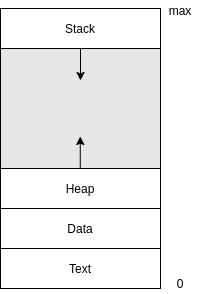
\includegraphics[width=4.5cm]{./assets/process.png}}
\vspace{.5cm}

Its parts are:
\begin{itemize}
	\item \textbf{Stack}
	\vspace{.2cm} \\
	It is a dynamically allocated memory which is used to hold temporary data, such as parameters and local variables.
	
	\item \textbf{Heap}
	\vspace{.2cm} \\
	Is memory that is dynamically allocated during process run time.
	
	\item \textbf{Data}
	\vspace{.2cm} \\
	Contains global variables.
	
	\item \textbf{Text}
	\vspace{.2cm} \\
	It represents the textual part of the process (i.e. the code).
\end{itemize}
A \textbf{program} is a passive entity, often referred to as an executable file. On the other hand, a \textbf{process} is an active entity.

\subsection{Process States}
A process during its lifetime may change state. A state diagram corresponding to each of the possible states could be: \\ \\

\centerline{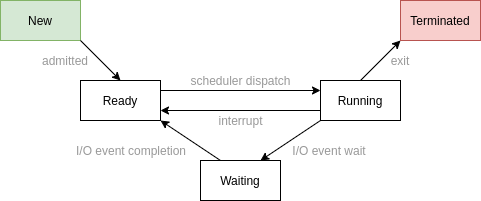
\includegraphics[width=11cm]{./assets/state.png}}
\vspace{.5cm}
The states are:

\begin{itemize}
	\item \textbf{New}
	\vspace{.2cm} \\
	The process is being created.
	
	\item \textbf{Running}
	\vspace{.2cm} \\
	Instructions are being executed.
	
	\item \textbf{Waiting}
	\vspace{.2cm} \\
	The process is waiting for some event to occur.
	
	\item \textbf{Ready}
	\vspace{.2cm} \\
	Waiting for the process to be assigned to a processor.
	
	\item \textbf{Terminated}
	\vspace{.2cm} \\
	The process has finished to execute.
\end{itemize}

\subsection{Process Control Block}
Each process is represented in the operating system by a \textbf{PCB} (Process Control Block). The PCB includes the following information about a process:

\begin{itemize}
	\item \textbf{Process State}
	
	\item \textbf{Program Counter}
	\vspace{.2cm} \\
	It indicates the address of the next instruction to be executed for this process.
	
	\item \textbf{CPU Registers}
	\vspace{.2cm} \\
	This information must be saved when an interrupt occurs, in order to allow the process to be continued correctly afterwards.
	
	\item \textbf{CPU-Scheduling Information}
	\vspace{.2cm} \\
	It includes process priority, pointers to scheduling queues, and other scheduling parameters.
	
	\item \textbf{Memory-Management Information}
	
	\item \textbf{Accounting Information}
	\vspace{.2cm} \\
	It includes the amount of CPU and real time used, time limits...
	
	\item \textbf{I/O Status Information}
	\vspace{.2cm} \\
	It includes a list of I/O devices allocated to the process, list of open files...
\end{itemize}

\subsection{Process Scheduling}
In order to obtain multiprogramming and time-sharing in a machine, the \textbf{process scheduler} selects an available process for program execution on the CPU.

\subsubsection{Scheduling Queues}
The following are the queues a process is put into when it enters the system:

\begin{itemize}
	\item \textbf{Job Queue}
	\vspace{.2cm} \\
	Queue containing all of the processes in the system.
	
	\item \textbf{Ready Queue}
	\vspace{.2cm} \\
	A set of all processes residing in main memory, ready and waiting to execute.
	
	\item \textbf{Device Queue}
	\vspace{.2cm} \\
	A set of processes waiting for an I/O device.
\end{itemize}
During their lifetime, processes can migrate among the various queues.

\subsubsection{Schedulers}
The operating system must select processes from the previously mentioned queues in some fashion. The selection process is carried out by the appropriate scheduler. There are three main schedulers:

\begin{itemize}
	\item \textbf{Long-Term Scheduler}
	\vspace{.2cm} \\
	Selects which process should be brought into the ready queue, by bringing them into memory. It also frequently controls the degree of multiprogramming within a system.
	
	\item \textbf{Short-Term Scheduler}
	\vspace{.2cm} \\
	Selects which process from the ready queue should be executed next and allocates the CPU.
	
	\item \textbf{Medium-Term Scheduler}
	\vspace{.2cm} \\
	Sometimes is advantageous to remove a process from execution in order to reduce the degree of multiprogramming. Later the process can be reintroduced into memory. This is also known as \textbf{swapping}.
\end{itemize}
The main difference between these first two schedulers is the frequency of execution. While the short-term scheduler is invoked very frequently, the long-term scheduler is instead invoked very infrequently. \\ \\
The long-term scheduler controls the degree of \textbf{multiprogramming}, i.e. the number of processes in memory. Most processes can be described as:

\begin{itemize}
	\item \textbf{I/O Bound Process}
	\vspace{.2cm} \\
	This is a process that spends most of its time doing I/O operations rather than computations.
	
	\item \textbf{CPU-Bound Process}
	\vspace{.2cm} \\
	This is a process that spends most of its time doing computations
\end{itemize}

\subsubsection{Context Switch}
When an interrupt occurs, the system needs to save the current \textbf{context} of the running process, so that it can be restored later. Generically, a \textbf{state save} of the current CPU is performed, and then a \textbf{state restore} in performed in order to resume operation. \\ \\
The constant switching of context is known as \textbf{content switching}, and it is pure overhead.

\subsection{Operation on Processes}

\subsubsection{Process Creation}
Parent processes can create children processes which in turn can create other children processes. This forms a tree of processes. \\ \\
A child process may be able to obtain its resources directly from the operating system, or it may be constraint to a subset of the resources of the parent process. Parent processes may also pass along some initialization data to the children processes. \\ \\
Two options are possible when processes are initiated, they can either run concurrently or the parent will wait for the children to finish executing. \\ \\
There are also two address-space possibilities for new processes. The first is that the child process is a duplicate of the parent process (same program and data as the parent). The second possibility is that the child process has a new program loaded into it. \\ \\
The following is a graph displaying what happens when a \cverb|fork()| method is called on a process: \\ \\

\centerline{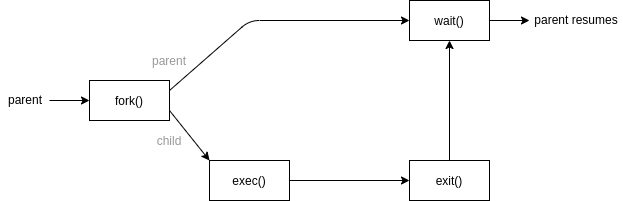
\includegraphics[width=11cm]{./assets/process creation.png}}
\vspace{.5cm}

\subsubsection{Process Termination}
A process terminates when it finishes executing its final statement and asks the OS to delete it by using the exit() system call. The process now may do the following:

\begin{itemize}
	\item Output data from child process to parent (via the \cverb|wait()| system call)
	\item All process resources are deallocated by the operating system.
\end{itemize}
A child process can also be terminated by using the \cverb|abort()| system call. This could happen for a variety of reasons:

\begin{itemize}
	\item The child exceeded the usage of some of the resources that it has been allocated
	\item The task assigned to the child is no longer required
	\item The operating system does not allow for a child to continue if its parent terminates. In this case, all child processes are killed (\textbf{cascading termination})
\end{itemize}
A \textbf{zombie process} is a process that has been terminated, but whose parent has not yet called \cverb|wait()| \\ \\
An \textbf{orphan process} is a child process that has not invoked \cverb|wait()|. Orphan processes are assigned \cverb|init| as their new parent process. The \cverb|init| process periodically invokes the \cverb|wait()| system call.

\subsection{Interprocess Communication}
A process is said to be \textbf{independent} if it cannot affect or be affected by the other processes executing in the system. \\ \\
A process, instead, is said to be \textbf{cooperating} if it affects and can be affected by the other processes executing in the system. \\ \\
Cooperating processes require an \textbf{interprocess communication mechanism} that will allow them to exchange data and information. There are two fundamental models of interprocess communication:

\begin{itemize}
	\item \textbf{Shared Memory}
	\vspace{.2cm} \\
	A region of memory that is shared by cooperating processes is established. Processes can then exchange information by reading and writing data to the shared region. This method is fast and no assistance from the kernel is required. It suffers though of cache coherency issues.
	
	\item \textbf{Message Passing}
	\vspace{.2cm} \\
	Communication takes place by means of messages exchanged between the cooperating processes. It is useful to exchange small amounts of data, and is easier to implement in a distributed system.
\end{itemize}

\subsubsection{Shared-Memory Systems}
In shared-memory systems a region of memory is shared in order to make multiple processes communicate with each other. In these systems there is a \textbf{producer} process that puts data into a buffer, and a \textbf{consumer} process that gets the data from this buffer. \\ \\
Two types of buffers can be used:

\begin{itemize}
	\item \textbf{Bounded Buffer}
	\vspace{.2cm} \\
	Assumes a fixed buffer size. In this case the consumer must wait if the buffer is empty, and the producer must wait if the buffer is full.
	
	\item \textbf{Unbounded Buffer}
	\vspace{.2cm} \\
	It places no limit on the actual size of the buffer. In this case the consumer has to wait if the buffer is empty, but the producer doesn't need to wait.
\end{itemize}

\subsubsection{Message-Passing System}
This system provides a mechanism to allow processes to communicate and to synchronize their actions without sharing the same address space. \\ \\
Message passing can be of two types:

\begin{itemize}
	\item \textbf{Blocking}
	\vspace{.2cm} \\
	This is considered \textbf{synchronous}. In \textbf{blocking send} operations, the sending process is blocked until the message is received by the receiving process. In \textbf{blocking receive} operations, the receiver blocks until a message is available.
	
	\item \textbf{Nonblocking}\
	\vspace{.2cm} \\
	This is considered \textbf{asynchronous}. In \textbf{nonblocking send} operations, the sending process sends the message and resumes operation. In \textbf{nonblocking receive} the receiver retrieves either a valid message or a null.
\end{itemize}

\subsection{Pipes}
A \textbf{pipe} acts as a conduit allowing two processes to communicate. Pipes are one of the first mechanisms in early UNIX systems.

\subsubsection{Ordinary Pipes}
\textbf{Ordinary pipes} allow two processes to communicate in standard producer-consumer fashion. The producer writes to the write-end of the pipe, while the consumer reads on the read-end of the pipe. \\ \\
These pipes are \textbf{unidirectional}. Two pipes must be used for bi-directional communication (in UNIX systems, \cverb|fd[0]| is the read-end, while \cverb|fd[1]| is the write-end). \\ \\
An ordinary pipe cannot be accessed from outside the process that created it. Here is a representation:

\begin{cverbatim}
      Parent                                           Child
  fd[0]    fd[1]                                   fd[0]   fd[1]
   |        |                                       |       |
   |        +---------------------------------------+---+   |
   |                                                |   |   |
   |    +-------------------------------------------+   |   |
   |    |                                               |   |
   |    |      +---------------------------------+      |   |
   |    +----> |                                 | <----+   |
   |           |              Pipe               |          |
   +---------> |                                 | <--------+
               +---------------------------------+
                
\end{cverbatim}

\subsubsection{Named Pipes}
Named pipes provide bi-directional communication, and no parent-child relationship is required. Once it has been established, a named pipe can be used by several processes. They also continue to exist after the communicating processes have finished.

\section{Multithreaded Programming}
\subsection{Thread}
A \textbf{thread} is a basic unit of CPU utilization. It comprises a thread ID, a program counter, a register set and a stack. It shares with other threads belonging to the same process its code section, data section and other operating system resources. \\ \\
A process can either be \textbf{single-threaded} or \textbf{multithreaded}. In this second case, the program can perform multiple tasks at the same time.

\subsection{Benefits}
There are some benefits that come with multithreaded programming, such as:

\begin{itemize}
	\item \textbf{Responsiveness}
	\vspace{.2cm} \\
	It may allow continued execution if part of the process is blocked, it is especially important for GUIs.
	
	\item \textbf{Resource Sharing}
	\vspace{.2cm} \\
	Threads share resources of the process, which is easier than both shared memory and message passing. The advantage is that an application can have several threads within the same address space.
	
	\item \textbf{Economy}
	\vspace{.2cm} \\
	Creating and context switching threads is generally faster than doing the same with processes.
	
	\item \textbf{Scalability}
	\vspace{.2cm} \\
	Process can take advantage of multiprocessor systems.
\end{itemize}

\subsection{Multicore Programming}
In a \textbf{multicore} system, multiple threads can run simultaneously in parallel. \\ \\
 A system is said to be \textbf{parallel} if it can perform more than one task simultaneously. On the other hand, a system is said to be \textbf{concurrent} if it supports more than one task by allowing all the tasks to make progress. \\ \\
It is possible to have concurrency without parallelism. \\ \\
The main challenges in programming for multicore systems are:

\begin{itemize}
	\item \textbf{Identifying Tasks}
	\vspace{.2cm} \\
	This involves examining applications to find areas that can be divided into separate, concurrent tasks.
	
	\item \textbf{Balance}
	\vspace{.2cm} \\
	While identifying tasks that can run in parallel, it must also be ensured that the tasks perform equal work of equal value.
	
	\item \textbf{Data Splitting}
	\vspace{.2cm} \\
	The data accessed and manipulated by the tasks must be divided to run on multiple cores.
	
	\item \textbf{Data Dependency}
	\vspace{.2cm} \\
	The data accessed by the tasks must be examined for dependencies between two or more tasks.
	
	\item \textbf{Testing and Debugging}
\end{itemize}
There are two main types of parallelism:

\begin{itemize}
	\item \textbf{Data Parallelism}
	\vspace{.2cm} \\
	It focuses on distributing subsets of the same data across multiple computing cores and performing the same operation on each core.
	
	\item \textbf{Task Parallelism}
	\vspace{.2cm} \\
	It involves distributing tasks across multiple cores. Each thread is performing a unique operation.
\end{itemize}

\subsection{Multithreading Models}
Support for threads might be provided at two levels:

\begin{itemize}
	\item \textbf{User Threads}
	\vspace{.2cm} \\
	Are supported above the kernel and are managed without the kernel's support.
	
	\item \textbf{Kernel Threads}
	\vspace{.2cm} \\
	Are supported and managed directly by the operating system.
\end{itemize}
There is a relationship between user and kernel threads. Following are three common ways of establishing such relationships.

\subsubsection{Many-to-One Model}
This model maps \textbf{many user threads} to \textbf{one kernel thread}. \\ \\
This is efficient, but the system halts whenever a blocking system call is executed. In this model threads are unable to run in parallel on multicore systems.

\subsubsection{One-to-One Model}
This model maps \textbf{each user thread} with \textbf{one kernel thread}. \\ \\
It has a degree of concurrency and threads can run in parallel. There is the overhead of creating the kernel thread corresponding to a user thread.

\subsubsection{Many-to-Many Model}
This model multiplexes \textbf{many user threads} to a \textbf{smaller or equal number of kernel threads}. \\ \\
This allows greater concurrency. If a user thread executes a blocking system call, the kernel can schedule another thread for execution.

\subsection{Threading Issues}
When working with threads, a series of issues can present to the developer. These are:

\begin{itemize}
	\item \textbf{fork() and execute() System Calls}
	\vspace{.2cm} \\
	There are two different versions of the \cverb|fork()| method. The first one duplicates all threads, while the other only duplicates only the threads that invoked \cverb|fork()|. \\ \\
	If a thread invokes the \cverb|exec()| system call, the program specified in the parameter of \cverb|exec()| will replace the entire process (including all of its threads).
	
	\item \textbf{Signal Handling}
	\vspace{.2cm} \\
	A \textbf{signal} is used in UNIX to notify a process that a particular event has occurred. A signal can be received either synchronously or asynchronously. \\ \\
	Signals can be either handled  by a default or user-defined signal handler. In multithreaded programs, delivering signals may be tricky. In the case of \textbf{synchronous signals}, they are only delivered to the thread causing the signal. In the case of \textbf{asynchronous signals}, the signal could either be delivered to all threads of the program, or only to one.
	
	\item \textbf{Thread Cancellation}
	\vspace{.2cm} \\
	This involves terminating a thread before it has completed. A thread that is to be canceled is referred to as the \textbf{target thread}. \\ \\
	There are two ways in which a thread can be canceled:
	
	\begin{itemize}
		\item \textbf{Asynchronous Cancellation}
		\vspace{.2cm} \\
		One thread immediately terminates the target thread.
		
		\item \textbf{Deferred Cancellation}
		\vspace{.2cm} \\
		The target thread periodically checks whether it should terminate, allowing it to terminate itself.
	\end{itemize}
	The problem with thread cancellation are the allocated resources. In case of asynchronous cancellation, sometimes it may occur that the OS, while reclaiming all system resources from a thread, does not actually reclaim all of them.
\end{itemize}

\subsection{Thread-Local Storage}
In some circumstances, threads need its own copy of certain data. this data is called \textbf{TLS} (Thread-Local Storage). \\ \\
Unlike local variables that are visible only during a single function invocation, TLS data are visible across function invocations.

\subsection{Scheduler Activations}
An intermediate data structure is implemented between the user and the kernel threads. This data structure, also known as \textbf{LWP} (LightWeight Process) is used for communication between the kernel and the thread library. This communication is also known as \textbf{scheduler activation}. \\ \\
To the user-thread library, the LWP appears to be a virtual processor on which the application can schedule a user thread to run. If a kernel thread blocks, the LWP blocks as well. A user thread attached to that LWP would block too.

\section{Process Scheduling}
\subsection{CPU-I/O Burst Cycle}
Process execution consists of a cycle of a CPU execution and an I/O wait. The process execution begins with a CPU burst.

\subsection{CPU Scheduler}
Whenever the CPU becomes idle, the operating system must select one of the processes in the ready queue to be executed. The scheduler's job is to select a process from the processes in memory which are ready to execute and allocate the CPU to that process. \\ \\
If a process switches from running to waiting state or from running to ready state, \textbf{nonpreemptive schedulers} are used. Instead, when a process switches from waiting to ready or it terminates, then \textbf{preemptive schedulers} are used. \\ \\
A \textbf{dispatcher} is involved in CPU-scheduling. It is a module that gives control of the CPU to the process selected by the short term scheduler. The operations involved are:

\begin{itemize}
	\item \textbf{Context Switching}
	\item \textbf{Switching to User-mode}
	\item \textbf{Jumping to the proper location in the user program in order to restart it}
\end{itemize}
The time it is needed for the dispatcher to stop one process and start another is known as the \textbf{dispatch latency}.

\subsection{Scheduling Criteria}
The following are the criteria used in order to compare CPU-scheduling algorithms -- following each parameter is which quantity of that measurement is best:

\begin{itemize}
	\item \textbf{CPU Utilization} - Max
	\vspace{.2cm} \\
	Keep the CPU as busy as possible.
	
	\item \textbf{Throughput} - Max
	\vspace{.2cm} \\
	Number of processes that complete their execution per time unit.
	
	\item \textbf{Turnaround Time} - Min
	\vspace{.2cm} \\
	The amount of time needed to execute a particular process.
	
	\item \textbf{Waiting Time} - Min
	\vspace{.2cm} \\
	The amount of time a process has been waiting for inside of the ready queue.
	
	\item \textbf{Response Time} - Min
	\vspace{.2cm} \\
	The amount of time that passes from the submission of a request until the first response is produced.
\end{itemize}

\subsection{Length of the Next CPU Burst}
The length of the next CPU burst can be calculated by using the length of previous CPU bursts, using exponential averaging. The following is the formula: \

\[ \tau_{n+1} = \alpha \cdot t_n + (1-\alpha) \cdot \tau_n \] \\
Were $t_n$ is the actual length of the n$^{\text{th}}$ CPU burst, while $\tau_{n+1}$ is the value for the next CPU burst.

\subsection{Scheduling Algorithms}
There are many scheduling algorithms, each having its upsides and downsides. Here are some of them.

\subsubsection{FCFS Scheduling}
\textbf{FCFS} (First Come, First Served) is the simplest CPU-scheduling algorithm that one can implement. The processes are simply scheduled based on their time of arrival in the ready queue.
\\
\begin{cverbatim}
 Arrival times:
  - P1 (burst time: 24)
  - P2 (burst time: 3)
  - P3 (burst time: 3)
\end{cverbatim}
\
\begin{cverbatim}
 Scheduling:
 +-----------------------------------+------------+------------+
 |                P1                 |     P2     |     P3     |
 +-----------------------------------+------------+------------+
 |                                   |            |            |
 0                                   24           27           30
 \end{cverbatim}
 
 \begin{cverbatim}
 Waiting times:
  - P1 = 0
  - P2 = 24
  - P3 = 27
    -------
    Avg. 17
\end{cverbatim}
Here we have what is known as the \textbf{convoy effect}, where the short processes are slowed down by the longer processes executing before them.

\subsubsection{SJF Scheduling}
\textbf{SJF} (Shortest Job First) associates with each process the length of the process's next CPU burst. These lengths are used to schedule the process with the shortest time. In this case it is non-preemptive.
\\
\begin{cverbatim}
 Arrival times:
  - P1 (burst time: 6)
  - P2 (burst time: 8)
  - P3 (burst time: 7)
  - P4 (burst time: 3)
\end{cverbatim}
\
\begin{cverbatim}
 Scheduling:
 +--------+------------+----------------+----------------------+
 |   P4   |     P1     |       P3       |          P2          |
 +--------+------------+----------------+----------------------+
 |        |            |                |                      |
 0        3            9                16                     24
\end{cverbatim}
\
\begin{cverbatim}
 Waiting times:
  - P1 = 3
  - P2 = 16
  - P3 = 9
  - P4 = 0
    -------
    Avg. 7
\end{cverbatim}
\
\subsubsection{SRTF Scheduling}
\textbf{SRTF} (Shortest Remaining Time First) is the preemptive version of the SJF algorithm. In this case the execution of one process can be interrupted by the CPU.

\begin{cverbatim}
 Arrival times:
  - P1 - 0 (burst time: 8)
  - P2 - 1 (burst time: 4)
  - P3 - 2 (burst time: 9)
  - P4 - 3 (burst time: 5)
\end{cverbatim}
\
\begin{cverbatim}
 Scheduling:
 +----+--------+------------+--------------+-------------------+
 | P1 |   P2   |     P3     |      P1      |        P3         |
 +----+--------+------------+--------------+-------------------+
 |    |        |            |              |                   |
 0    1        5            10             17                  26
\end{cverbatim}
\
\begin{cverbatim}
 Waiting times:
  - P1 = 10-1 = 9
  - P2 = 1-1 = 0
  - P3 = 17-2 = 15
  - P4 = 5-3 = 2
    --------------
    Avg. 6.5
\end{cverbatim}
\
\subsubsection{Priority Scheduling}
In the case of \textbf{priority scheduling}, a priority number is assigned to each process.
\\
\begin{cverbatim}
 Priorities:
  - P1 - 3 (burst time: 10)
  - P2 - 1 (burst time: 1)
  - P3 - 4 (burst time: 2)
  - P4 - 5 (burst time: 1)
  - P5 - 2 (burst time: 5)
\end{cverbatim}
\
\begin{cverbatim}
 Scheduling:
 +----+--------+-----------------------+------------+----------+
 | P2 |   P5   |          P3           |     P1     |    P4    |
 +----+--------+-----------------------+------------+----------+
 |    |        |                       |            |          |
 0    1        6                       16           18         19
\end{cverbatim}
\
\begin{cverbatim}
 Waiting times:
  - P1 = 16
  - P2 = 0
  - P3 = 6
  - P4 = 18
  - P5 = 1
    --------
    Avg. 8.2
\end{cverbatim}
\
\subsubsection{RR Scheduling}
\textbf{RR} (Round Robin) is a scheduling algorithm in which each process gets a small unit of CPU time -- usually from 10 to 100 milliseconds. After this time has elapsed, the process is preempted and is added to the end of the ready queue.
\\
\begin{cverbatim}
 Arrival times:
  - P1 (burst time: 53)
  - P2 (burst time: 17)
  - P3 (burst time: 68)
  - P4 (burst time: 24)
  
 Time quantum: 20 
\end{cverbatim}
\
\begin{cverbatim}
 Scheduling:
 +-----+-----+-----+-----+-----+-----+-----+-----+-----+-------+
 | P1  | P2  | P3  | P4  | P1  | P3  | P4  | P1  | P3  |  P3   |
 +-----+-----+-----+-----+-----+-----+-----+-----+-----+-------+
 |     |     |     |     |     |     |     |     |     |       |
 0     20    37    57    77    97   117   121   134   154     162
\end{cverbatim}
\
\begin{cverbatim}
 Waiting Time:
  - P1 = 57+24 = 81
  - P2 = 20
  - P3 = 37+40+17 = 94
  - P4 = 57+40 = 97
  --------------------
  Avg. 73
\end{cverbatim}
\
\subsubsection{Multilevel Queue}
Here the ready queue is permanently partitioned into two distinct queues, based on certain properties of the process. For example memory size, process priority or process size. A common partitioning is:

\begin{itemize}
	\item \textbf{Foreground} - Interactive $\rightarrow$ RR Scheduling
	\item \textbf{Background} - Batch $\rightarrow$ FCFS Scheduling
\end{itemize}
In a multilevel queue system, each queue has absolute priority over lower-priority queues.

\subsubsection{MLFQ Scheduling}
\textbf{MLFQ} (MultiLevel Feedback Queue) is a scheduling algorithm where a process can move between the various queues. In general, a MLFQ scheduler is defined by the following parameters:

\begin{itemize}
	\item Number of queues
	\item Scheduling algorithms for each queue
	\item Method used to determine when to upgrade a process
	\item Method used to determine when to demote a process
	\item Method used to determine which queue a process will enter when that process needs service
\end{itemize}

\subsubsection{Thread Scheduling}

When systems support threads, these are scheduled, not processes. In many-to-one and many-to-many models, the thread library schedules the user threads to run on LWPs. This is known as \textbf{PCS} (Process Contention Scope) since scheduling competition is within the process. \\ \\
Scheduling kernel threads onto available CPU is known as \textbf{SCS} (System-Contention Scope) since scheduling competition is among all threads in the system.

\subsubsection{Multi-Processor Scheduling}
When working with multiple processors, \textbf{load sharing} becomes possible. In this case scheduling algorithms become more and more complex. There are two main approaches when dealing with multi-processor scheduling:

\begin{itemize}
	\item \textbf{Asymmetric Multiprocessing}
	\vspace{.2cm} \\
	Only one processor is able to access the system data structures, thus alleviating the need of data sharing.
	
	\item \textbf{Symmetric Multiprocessing}
	\vspace{.2cm} \\
	Each processor is self-scheduling. All of the processes are either in a common queue, or each processor has its own queue of ready processes.
\end{itemize}

\subsection{Algorithm Evaluation}
In order to choose the best CPU-scheduling algorithm for a specific system or case, we need to test them in order to see which one is the most appropriate. There are several techniques that can be used in order to evaluate an algorithm.

\subsubsection{Deterministic Modeling}
In this evaluation, the scheduling algorithms take a predefined workload and is defined by the performance for that workload. \\ \\
This method is very simple, fast, and offers a direct comparison between the algorithms. But it is specific for an input.

\subsubsection{Queuing Models}
The distribution of CPU and I/O bursts is calculated and used to determine the performance of a scheduling algorithm. \\ \\
In order to analyze the algorithm, we can use \textbf{Little's Formula}, which is the following:

\[ n = \lambda \cdot W \] \\
Where $n$ is the average queue length, $\lambda$ is the average arrival time at the queue, and $W$ is the average waiting time. This formula is particularly useful, because it is valid for any scheduling algorithm and any arrival distribution. \\ \\
This method is more general than the deterministic modeling. But it can be difficult to handle, especially for complex distributions.

\subsubsection{Simulations}
In this case we use a simplified programming model of the actual computer system. The workload is synthetic and based on distributions. The data collected is empirical, meaning that is based on actual system measurements. \\ \\
This method is a faithful representation of the environment, but simpler. The problems with this approach are that the results may be inaccurate (if the model is over simplistic), or it can be computationally expensive or complex to program (if the model is too detailed).

\subsubsection{Implementation}
In this method the algorithm is directly introduced into the existing operating system. Here the algorithm is evaluated with a real environment and workload. \\ \\
This method is the ultimate representation of environment, where no detail is left out. But it could be very difficult to implement, and the result depends on the representative workload.

\section{Synchronisation}
A process is said to be \textbf{cooperating} if it can be affected by or can affect other processes executing in the system. These processes can either directly share a logical space, or they can be allowed to share data only through files or messages.

\subsection{The Critical Section Problem}
A \textbf{critical section} is a section of code in which the process may be changing common variables, writing a file... \\ \\
In order to find a solution to the critical section problem, the following requests must be satisfied:

\begin{itemize}
	\item \textbf{Mutual Exclusion}
	\vspace{.2cm} \\
	If a process $P_i$ is executing a critical section, then no other process can be executing that critical section.
	
	\item \textbf{Progress}
	\vspace{.2cm} \\
	If no process is executing in its critical section, and there exist some processes that wish to enter their critical section, then the selection of the process that will enter its critical section next cannot be indefinitely postponed.
	
	\item \textbf{Bounded Waiting}
	\vspace{.2cm} \\
	A bound must exist on the number of times that other processes are allowed to enter their critical section, after a process has made a request to enter its critical section and before the request has been granted.
\end{itemize}
In operating systems, two techniques are mainly used in order to handle critical sections:

\begin{itemize}
	\item \textbf{Preemptive Kernel}
	\vspace{.2cm} \\
	This allows a process to be stopped while it's running in kernel mode.
	
	\item \textbf{Non-preemptive Kernel}
	\vspace{.2cm} \\
	This doesn't allow a process to be stopped while it's running in kernel mode.
\end{itemize}

\subsection{Peterson's Solution}
This solution is restricted to two processes that alternate their execution between their critical sections and the remainder sections. These two processes share two data items:

\begin{itemize}
	\item \textbf{Turn}
	\vspace{.2cm} \\
	This decides whose turn is it to enter its critical section.
	
	\item \textbf{Flag[i]}
	\vspace{.2cm} \\
	It indicates if a process is ready to enter its critical section.
\end{itemize}

\subsection{Synchronization Hardware}
\textbf{Locking} is the action of protecting critical regions trough the use of locks. \\ \\
\textbf{Atomic hardware instructions} are those implemented in modern machines in order to provide solutions to the critical section problem.

\subsection{Semaphores}
A \textbf{semaphore} is a synchronization tool that does not require busy waiting. There are two atomic operations provided to modify a semaphore:

\begin{itemize}
	\item \cverb|wait()|
	\item \cverb|signal()|
\end{itemize}

\subsection{Monitors}
\textbf{Monitors} are a high level synchronization tool that provide a convenient and effective mechanism for process synchronization. Only one process may be active within the monitor at a time.

\subsection{Deadlocks and Starvation}
A \textbf{deadlock} happens when two or more processes are waiting indefinitely for an event that can be caused by only one of the waiting processes. \\ \\
\textbf{Starvation} is when a process may never be removed from the semaphore queue in which it is suspended.

\section{Memory Management Strategies}
In order for a program to be run, it must first be loaded into memory and placed within a process. \\ \\
The CPU can only access main memory and registers directly. The memory unit only sees a stream of addresses and read requests, or addresses, data and read requests. \\ \\
In order for a correct operation of the system, memory protection is required.

\subsection{Address Binding}
The binding of instructions and data to memory addresses can happen at three different stages:

\begin{itemize}
	\item \textbf{Compile Time}
	\vspace{.2cm} \\
	If a memory location is known beforehand, an absolute code can be generated. The code must be recompiled whenever the starting location changes.
	
	\item \textbf{Load Time}
	\vspace{.2cm} \\
	If the memory location is not known at compile time, then a relocatable code must be generated.
	
	\item \textbf{Execution Time}
	\vspace{.2cm} \\
	If the process can be moved during its execution from one memory segment to another, then address binding must be delayed until run time. In order for this to work, special hardware is needed.
\end{itemize}

\subsection{Logical vs Physical Address Space}
The \textbf{Logical address} is the address generated by the CPU. It is also referred to as virtual address. \\ \\
The \textbf{Physical address} is the address seen by the memory unit, and the one loaded into the memory-access register of memory. \\ \\
\textbf{Compile-time} and \textbf{load-time} methods generate identical logical and physical addresses. \textbf{Execution-time} address-binding scheme results in different logical and physical addresses.

\subsection{MMU (Memory Management Unit)}
MMU in a hardware device that maps virtual to physical addresses. In the MMU scheme, the value in the relocation register is added to every address generated by user processes. \\ \\
The user program only deals with logical addresses. It never sees the real physical address.

\subsection{Contiguous Allocation}
Main memory is usually divided in two partitions:

\begin{itemize}
	\item \textbf{Low Memory}
	\vspace{.2cm} \\
	It contains the resident operating system and the interrupt vector.
	
	\item \textbf{High Memory}
	\vspace{.2cm} \\
	It contains the user processes
\end{itemize}
Usually, it is desired for multiple user processes to reside in memory at the same time. In contiguous memory allocation, each process is contained in a single section of memory that is contiguous to the section containing the next process.

\subsection{Memory Protection}
A \textbf{relocation-register scheme} is used in order to protect users from accessing each others' files, and from changing operating-system code and data. \\ \\
The \textbf{relocation register} contains the value of the smallest physical address. \\ \\
Thew \textbf{limit register} contains a range of logical addresses. each logical address must be less than the limit register. \\ \\ \\

\centerline{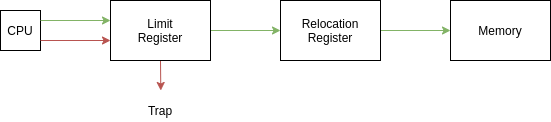
\includegraphics[width=10cm]{./assets/mem-protection.png}}

\subsection{Memory Allocation}
\subsubsection{Multiple Partition Allocation}
One of the simplest methods of allocating memory is to divide it into several fix-sized partitions. In the multiple-partition method, when a partition is free, a process is selected from the input queue and is loaded into the free partition. \\ \\
A \textbf{hole} is a block of available memory. When a process arrives, memory is allocated inside of a hole large enough to accommodate it. \\ \\
The Operating system always maintains information about the allocated and free partitions. \\ \\ \\

\centerline{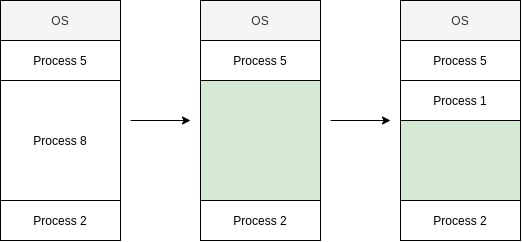
\includegraphics[width=10cm]{./assets/mult-partition.png}}
\vspace{.4cm}

\subsubsection{Dynamic Storage-Allocation Problem}
This problem concerns how to satisfy a request of size $n$ from a list of free holes. Some possible solutions to this problem are:

\begin{itemize}
	\item \textbf{First-Fit}
	\vspace{.2cm} \\
	Allocate the first hole that is big enough to fit the process.
	
	\item \textbf{Best-Fit}
	\vspace{.2cm} \\
	Allocate the smallest hole that is big enough. The whole list must be searched (unless it is ordered by size). It produces the smallest leftover hole.
	
	\item \textbf{Worst-Fit}
	\vspace{.2cm} \\
	Allocate the largest hole. The whole list must be searched (unless it is ordered by size). It produces the largest leftover hole.
\end{itemize}
In terms of speed and storage utilization, the first two options are best.

\subsection{Fragmentation}
\subsubsection{External Fragmentation}
Both first-fit and best-fit suffer from \textbf{external fragmentation}. As the processes are loaded and removed from memory, the free memory is broken down into smaller pieces. External fragmentation exists when there is enough total memory space to satisfy a request, but the available spaces are not continuous. This leaves free gaps in memory. \\ \\
Statistical analysis on first-fit shows that, given $n$ allocated blocks, $\frac{1}{2}n$ blocks will be lost to external fragmentation.

\subsubsection{Internal Fragmentation}
In the case of a multiple-partition allocation scheme, consider a hole of 1249 bytes. If we allocate 1247 bytes, then we are left with just 2 bytes. These 2 bytes are not enough to keep track of the hole. In order to solve this problem, the memory allocated to the process may be larger than the requested memory. The difference between these two numbers is known as \textbf{internal fragmentation}. \\ \\
A solution to internal fragmentation is given by \textbf{compacting} the memory. This consists in shuffling the memory content in order to place all of the free memory together in one large block. This is possible only with dynamic relocation. It is also done at execution time.

\subsection{Swapping}
A process can be swapped temporarily out of memory to a backing store. Then this process is brought back into memory for continued execution. \\ \\
A \textbf{backing store} is a fast disk that is large enough to accommodate copies of all memory images for all users. It must provide direct memory access to those images. \\ \\
Most of the swap time is transfer time. The total transfer time is directly proportional to the amount of memory swapped.

\subsection{Paging}
\textbf{Paging} is another memory-management technique that permits the physical address space of a process to be non-contiguous. This scheme avoids external fragmentation, and thus the need of compacting memory. \\ \\
In order to implement paging, physical memory is broken down into fixed-size blocks called \textbf{frames}. Logical memory is also divided into blocks of the same size called \textbf{pages}. \\ \\
A page number is used as an index into a \textbf{page table}. This table contains the base address of each page in physical memory. This base address is combined with the page offset in order to define the physical memory address sent to the memory unit. \\ \\
The address generated by the CPU is divided into:

\begin{itemize}
	\item \textbf{Page Number}
	\vspace{.2cm} \\
 	The page number is used as an index into a page table.
 	
 	\item \textbf{Page Offset}
 	\vspace{.2cm} \\
 	The page offset is combined with a base address to define the physical memory address that is sent to the memory unit.
\end{itemize}

\subsubsection{Page Table}
A page table is kept into main memory. It has a \textbf{PTBR} (Page-Table Base Register) that indicates the size of the page table. By doing so, every data or instruction access requires two memory addresses: one for the page table and one for the data/instruction. \\ \\
These memory access problems can be solved by means of a special fast-lookup hardware cache, called a \textbf{TLB} (Translation Look-aside Buffer).

\subsubsection{Effective Access Time}
The formula for the EAT is:

\[ EAT = 2 + \varepsilon - \alpha \]
Where $\alpha$ is the hit ratio, which is the percentage of times that a page number is found in the associative registers, and $\varepsilon$ is the associative lookup time unit.

\subsubsection{Memory Protection}
Memory protection is implemented by associating a protection bit with each frame. This valid/invalid bit is attached to every entry in the page table. The two states of the protection bit are:

\begin{itemize}
	\item \textbf{Valid}
	\vspace{.2cm} \\
	The associated page is in the processes' logical address space, making it a legal page.
	
	\item \textbf{Invalid}
	\vspace{.2cm} \\
	The page is not in the processes' logical address space.
\end{itemize}

\subsubsection{Shared Pages}
One copy of read-only code is shared among processes. This shared code must appear in the same location in the logical addresses space of all processes. \\ \\
Each process keeps a separate copy of the code and data. The pages for the copied code and data can appear anywhere in the logical address pace of the processor.

\subsection{Page Table Structures}
There are several ways to structure tables in memory. Three of them are:

\begin{itemize}
	\item \textbf{Hierarchical Page Tables}
	\vspace{.2cm} \\
	In this case the logical address space is broken up into multiple page tables. One simple example is a \textbf{two-level page table}. Here the address is divided into a page number, the offset of the inner page, and the offset of the outer page.
	
	\item \textbf{Hashed Page Table}
	\vspace{.2cm} \\
	A virtual page number is hashed into a page table. This page table contains a chain of elements hashing to the same location. The page numbers are compares with the elements of the hashed chain. If a match is found, then the corresponding physical address is extracted.
	
	\item \textbf{Inverted Page Table}
	\vspace{.2cm} \\
	One entry is set for each real page of memory. This entry consists of the virtual address of the page stored in that real memory location, with information about the process that owns that page. \\ \\
	This method is more efficient in terms of memory needed to store each page table, but also more inefficient in terms of access time.
\end{itemize}

\subsection{Segmentation}
Segmentation is a memory management scheme that supports a user view of memory. A program is a collection of segments. A segment is a \textbf{logical unit}. \\ \\
A logical address consists of a two-tuple made up by:

\begin{itemize}
	\item \textbf{Segment Number}
	\item \textbf{Offset}
\end{itemize}
A segment table job is to map two-dimensional physical addresses. Each of the table entries have:

\begin{itemize}
	\item \textbf{Base}
	\vspace{.2cm} \\
	Contains the starting physical address where the segment resides in memory.
	
	\item \textbf{Limit}
	\vspace{.2cm} \\
	Specifies the length of the segment.
\end{itemize}
There are two types of registers, the first is the \textbf{STBR} (Segment-Table Based Register), that points to the segment table's location in memory. \\ \\
The second register is the \textbf{STLR} (Segment-Table Length Register), that points to the number of segments used by a program. The segment number is legal iff it is strctly less that \textbf{STLR}. \\ \\
In the segmentation architecture, three main operations are possible:

\begin{itemize}
	\item \textbf{Relocation}
	\item \textbf{Sharing}
	\item \textbf{Allocation}
\end{itemize}
With each entry of the segment table is associated a validation bit and read/write/execute privileges. \\ \\
Since segments can vary in length, memory allocation is a dynamic storage-allocation problem.

\section{Virtual Memory}
It is the separation of the user logical memory from physical memory. Virtual memory offers many advantages, such as:

\begin{itemize}
	\item Only part of the program needs to be in memory in order to be executed.
	\item Logical address space can be much larger than physical address space.
	\item Allows the address spaces to be shared by several processes.
	\item Allows for more efficient process creation.
\end{itemize}

\subsection{Demand Paging}
This is a way used to implement virtualization. Pages are brought into memory only when needed. This introduces many advantages, such as:

\begin{itemize}
	\item Less I/O is needed
	\item Less memory is needed
	\item Faster response times
	\item More users possible
\end{itemize}
When a page is needed, a reference to it is created. In the case of an invalid reference, abort. Otherwise, if the referenced page is not in memory, it must first be brought into memory.

\subsection{Valid-Invalid Bit}
With each table entry is associated a valid-invalid bit (1 $\rightarrow$ in memory, 0 $\rightarrow$ not in memory). This bit is initially set to 0 on all entries. \\ \\
If during the address translation, the valid-invalid bit is set to 0, we have a \textbf{page fault}.

\subsection{Page Fault}
A page fault happens if the page that is trying to access has its valid-invalid bit set to 0 (the page is not in memory). The following are the steps followed in order to handle the page fault:

\begin{enumerate}
	\item A trap occurs, which alerts the OS that the requested page is not in main memory.
	\item The page is looked for in the backing storage.
	\item The page is brought into main memory, the table is reset, and the valid-invalid bit for that entry is set to 1 (i.e. the page is now in memory).
	\item The instruction is restarted.
\end{enumerate}
In the case there were no free frames, a page in memory that is not being used is swapped out.

\subsection{Process Creation}
Virtual memory also allows advantages when creating processes, such as:

\begin{itemize}
	\item \textbf{Copy-on-Write}
	\vspace{.2cm} \\
	This method allows both the parent and the child process to share the same pages in memory. \\ \\
	The page in this case is copied only when it is modified by one between the parent and the child.
	
	\item \textbf{Memory-Mapped Files}
\end{itemize}

\subsection{Page Replacement}
This method is used in order to prevent the over-allocation of memory. A \textbf{dirty bit} is introduced in order to reduce the overhead of page transfers -- only modified pages are written onto the disk. \\ \\
Page replacement completes the separation between logical and physical memory. Large virtual memory can be provided on smaller physical memory. \\ \\
Here are the steps that are followed in order to perform a page replacement:

\begin{itemize}
	\item Find the location of the desired page on the disk.
	\item Find a free frame. In the case there is no free frame, a replacement algorithm is used in order to select the page to be swapped.
	\item The page is read into the newly free frame. Both the page and the free frame tables are updated.
	\item The process is restarted.
\end{itemize}

\subsection{Page Replacing Algorithms}
The ultimate goal of page replacement algorithms is to obtain the lowest possible page-fault rate.

\subsubsection{FIFO Algorithm}
The first element to be inserted is the first to one to be replaced. \\ \\
FIFO replacement leads to something known as \textbf{Belady's Anomaly}, where having more frames would lead to more page faults.

\subsubsection{LRU Algorithm}
LRU (Least Recently Used) will replace the page that has not been used for the longest period of time. In order to implement this algorithm, two methods are used:

\begin{itemize}
	\item \textbf{Counter Implementation}
	\vspace{.2cm} \\
	Every page entry has a counter. For every time the page is referenced, the OS clock count is copied into the counter field. \\ \\
	The page that has the highest clock counter is the one that is going to be replaced first.
	
	\item \textbf{Stack Implementation}
	\vspace{.2cm} \\
	The records are put in a stack. The least recently used will be at the bottom of said stack. This stack is implemented as a doubly linked list, so it will be easier to get the first element.
\end{itemize}
The following are some methods used in order to decide which page to choose:

\begin{itemize}
	\item \textbf{Reference Bit}
	\vspace{.2cm} \\
	To each page is associated a bit -- which is initially 0. When a page is referenced, the reference bit is set to 1. \\ \\
	The page with reference bit 0 will be the one to be replaced.
	
	\item \textbf{Second Chance}
	\vspace{.2cm} \\
	A reference bit is needed. Furthermore, a clock replacement is used. If the page needs to be replaced and the bit is set to 1, then:
	
	\begin{enumerate}
		\item Set the reference bit to 0.
		\item Leave the page in memory.
		\item Restart the procedure for the next page in clock order.
	\end{enumerate}
\end{itemize}

\subsection{Counting Algorithms}
A counter is kept for all the number of references that have been made of each page. Then one of the following two algorithms will be used:

\begin{itemize}
	\item \textbf{LFU Algorithm}
	\vspace{.2cm} \\
	Replaced the page that has been least frequently used (i.e. the one with the smallest count).
	
	\item \textbf{MFU Algorithm}
	\vspace{.2cm} \\
	The MFU (Most Frequently Used) algorithm is based on the argument that the page with the smallest clock count was probably just brought in and has yet to be used.
\end{itemize}

\subsection{Allocation of Frames}
Each process require a minimum number of pages. In order to allocate these pages, we can use different schemes.

\subsubsection{Fixed Allocation}
Fixed allocation can be of two types:

\begin{itemize}
	\item \textbf{Equal}
	\vspace{.2cm} \\
	A fixed number of frames are given to each process.
	
	\item \textbf{Dynamic}
	\vspace{.2cm} \\
	Allocation is done based on the size of the process, and is computed as follows:
	
	\[ p_i = \frac{s_i}{S} \cdot m \] \\
	Where $s_i$ is the size of process $p_i$, \textbf{S} is $\sum_i s_i$, and \textbf{m} is the total number of frames.
\end{itemize}

\subsubsection{Priority Allocation}
A proportional allocation scheme is used with priority rather than size. In the case that process $p_i$ generates a page fault, either one of its frames or one from processes with lower priority number is selected for replacement. \\ \\
There are two main scopes for replacement:

\begin{itemize}
	\item \textbf{Global Replacement}
	\vspace{.2cm} \\
	A frame is selected from the set of all frames, in some cases a frame from another process could also be taken.
	
	\item \textbf{Local Replacement}
	\vspace{.2cm} \\
	Each process can only select frames from its own set of allocated frames.
\end{itemize}

\subsection{Thrashing}
If a process does not have enough pages, then the page fault rate will be very high. This will actively lead to:

\begin{itemize}
	\item Low CPU utilization.
	\item The OS thinks it needs to increase the degree of multiprogramming.
	\item Another process is added to the system.
\end{itemize}
Thrashing happens when a process is busy swapping pages in and out of memory. It occurs because the sum of the size of the locality is greater than the total memory size.

\subsection{Working-Set Model}
A working-set window is a fixed number of page reference, and il denothed by $\Delta$. And is used in the following definition:

\[ WSS_i = \text{pages referenced in the most recent}~\Delta \] \\
Where $WSS_i$ is the \textbf{Workings-Set Size} of process $p_i$. Depending on $\Delta$:

\begin{itemize}
	\item If $\Delta$ is too small, it will not encompass the entire locality.
	\item If $\Delta$ is too large, it will encompass several localities.
	\item If $\Delta = \infty$, it will encompass the entire program.
\end{itemize}
Furthermore, we have that:

\[ D = \sum_i WSS_i \] \\
Which is the total demanded frames. If $D > m$, then thrashing happens. Thus as policy if $D > m$ the program is suspended.

\subsection{Memory-Mapped Files}
This allows the file I/O to be treated as routine memory access by mapping a disk block to a page in memory. \\ \\
The following are the steps taken in order to access such files:

\begin{enumerate}
	\item A file is initially read using demand paging.
	\item A page-size portion of the file is read from the file's subsystem into a physical page.
	\item Subsequent read/writes to/from memory are treated as ordinary memory accesses.
\end{enumerate}
Thanks to this method, several processes are allowed to map the same file in order for memory to be shared.

\subsection{Allocating Kernel Memory}
Allocation of kernel memory is treated differently from use memory. Kernel memory is allocated from a free-memory pool.

\subsection{Buddy System}
The memory is allocated from a fixed-size segment consisting of physically continuous pages. \\ \\
The memory is allocated using a power-of-2 allocator. When a smaller allocation is needed than available, then the current chunk is split into two \textbf{buddies} of the next-lower power of 2. \\ \\
The main advantage of using this method is to quickly coalesce smaller unused memory chunks into a larger chunk. On the other hand, there is the disadvantage of fragmentation.

\subsection{Slab Allocator}
A \textbf{slab} consists of one or more contiguous pages. A \textbf{cache} consists of one or more slabs. \\ \\
There is a single cache for each unique kernel data structure. When such a cache is created, it is filled with objects marked as free. These objects will be marked as used whenever structures are stored. \\ \\
If a slab is full of used objects, then the next object will be allocated from an empty slab. \\ \\
The benefits of this method include no fragmentation and faster memory-request satisfaction.

\subsection{Other Issues}
Other issues of these techniques include:

\begin{itemize}
	\item \textbf{Prepaging}
	\vspace{.2cm} \\
	Prepaging can be used to reduce the number of page faults that occur at process startup. The problem with this is that if these pages are unused, the I/O and memory resources will be wasted.
	
	\item \textbf{Page Size}
	\vspace{.2cm} \\
	Page-size selection must take into account the following: fragmentation, table size, I/O overhead and locality.
	
	\item \textbf{TLB Reach}
	\vspace{.2cm} \\
	This is the amount of memory accessible from the TLB. By increasing the page size, this may lead to an increase in fragmentation, as not all applications require a large page size.
	
	\item \textbf{I/O Interlock}
	\vspace{.2cm} \\
	Pages must be sometimes locked into memory.
\end{itemize}

\section{Mass-Storage Systems}
Magnetic disks provide bulk secondary storage for modern computers. Some of the terminology is:

\begin{itemize}
	\item \textbf{Transfer Rate}
	\vspace{.2cm} \\
	The rate at which data flows between the drive and the computer.
	
	\item \textbf{Positioning Time}
	\vspace{.2cm} \\
	The time needed for the drive to move the disk arm to the desired cylinder.
	
	\item \textbf{Rotational Latency}
	\vspace{.2cm} \\
	The time needed for the desired sector to rotate under the disk arm.
	
	\item \textbf{Head Crash}
	This is when the disk head makes contact with the disk surface.
\end{itemize}
Drives are attached to computers via I/O buses. These buses can be of several types, such as: EIDE, ATA, SATA... The host controller in the computer uses these buses in order to talk to the disk controller built into either the drive or the storage array. \\ \\
A disk is accessed as a large one-dimensional array of logical blocks. A \textbf{logical block} is the smallest unit of transfer.

\subsection{Disk Scheduling}
Access time in disk scheduling has two main components:

\begin{itemize}
	\item \textbf{Seek Time}
	\item \textbf{Rotary Latency}
\end{itemize}
The main objective of such algorithms is to minimize the \textbf{seek time}. \\ \\
The \textbf{disk bandwidth} is the total number of bytes transferred, divided by the total time between the first request for service and the completion of the last transfer.

\subsubsection{FCFS Scheduling}
\begin{cverbatim}
Queue: 98, 183, 37, 122, 14, 124, 65, 67
Start: 53
\end{cverbatim}
\vspace{.3cm}
\centerline{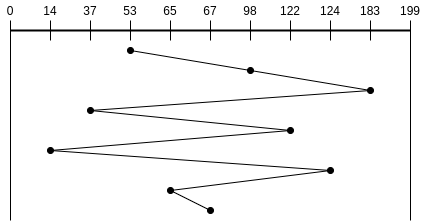
\includegraphics[width=9cm]{./assets/fcfs.png}}

\begin{cverbatim}
Total: (98-53)+(183-98)+(183-37)+(122-37)+(122-14)+(124-14)
       +(124-65)+(67-65) = 640 cylinders of head movement 
\end{cverbatim}

\subsubsection{SSTF Scheduling}
SSTF (Shortest Seek Time First) selects the request with the minimum seek time from the current head position. This is a form of SJF, and may cause starvation in some cases.

\begin{cverbatim}
Queue: 98, 183, 37, 122, 14, 124, 65, 67
Start: 53
\end{cverbatim}
\vspace{.3cm}
\centerline{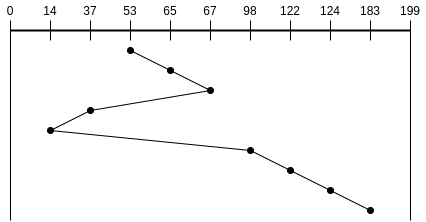
\includegraphics[width=9cm]{./assets/sstf.png}}
\vspace{.3cm}
\begin{cverbatim}
Total: (65-53)+(67-65)+(67-37)+(37-14)+(98-14)+(122-98)
       +(124-122)+(183-124) = 236 cylinders of head movement 
\end{cverbatim}

\subsubsection{SCAN Scheduling}
In SCAN scheduling, the disk arm starts from one end of the disk, and goes all the way to the other end.

\begin{cverbatim}
Queue: 98, 183, 37, 122, 14, 124, 65, 67
Start: 53
\end{cverbatim}
\vspace{.3cm}
\centerline{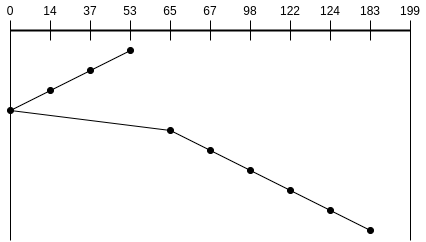
\includegraphics[width=9cm]{./assets/scan.png}}
\vspace{.3cm}
\begin{cverbatim}
Total: (53-37)+(37-14)+(65-14)+(67-65)+(98-67)+(122-98)
       +(124-122)+(183-124) = 208 cylinders of head movement 
\end{cverbatim}

\subsubsection{C-SCAN Scheduling}
C-SCAN scheduling provides a more uniform wait time than SCAN. It is like SCAN, but when it reaches the end of the disk, it quickly moves back to the beginning.

\begin{cverbatim}
Queue: 98, 183, 37, 122, 14, 124, 65, 67
Start: 53
\end{cverbatim}
\vspace{.3cm}
\centerline{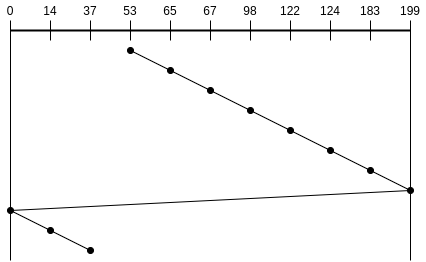
\includegraphics[width=9cm]{./assets/cscan.png}}
\vspace{.3cm}

\subsubsection{C-LOOK Scheduling}
This is a version of C-SCAN. In this case, the arm goes as far as the last request in each direction. Then, it reverses direction immediately.

\begin{cverbatim}
Queue: 98, 183, 37, 122, 14, 124, 65, 67
Start: 53
\end{cverbatim}
\vspace{.3cm}
\centerline{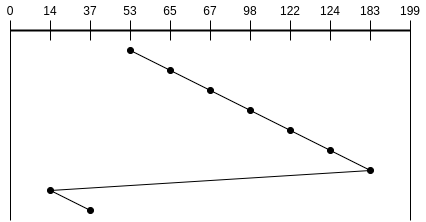
\includegraphics[width=9cm]{./assets/clook.png}}
\vspace{.3cm}

\section{File System Interface}
\subsection{File Concept}
A \textbf{file} is a contiguous logical address space. There are sever types of files, such as:

\begin{itemize}
	\item \textbf{Data}
	\vspace{.2cm} \\
	It can be numeric, composed of characters, or binary.
	
	\item \textbf{Program}
\end{itemize}

\subsubsection{File Structure}
A file can have a different structure based on the type of data it contains.

\begin{itemize}
	\item \textbf{None}
	If the file contains a sequence of words or bytes.
	
	\item \textbf{Simple Record Structure}
	\vspace{.2cm} \\
	For example lines of fixed or variable length.
	
	\item \textbf{Complex Structures}
	\vspace{.2cm} \\
	For example a formatted document or a relocatable load file.
\end{itemize}
Both the simple and complex structures can be simulated by the "None" structure by inserting the appropriate control characters.

\subsubsection{File Attributes}
A file can have several attributes, such as:

\begin{itemize}
	\item \textbf{Name}
	\vspace{.2cm} \\
	The only attribute that is kept in a human-readable form.
	
	\item \textbf{Identifier}
	\vspace{.2cm} \\
	A unique tag (represented by a number), which identifies the file within the file system.
	
	\item \textbf{Type}
	\vspace{.2cm} \\
	This attribute is needed for systems that support multiple file types.
	
	\item \textbf{Size}
	\vspace{.2cm} \\
	The size of the current file.
	
	\item \textbf{Protection}
	\vspace{.2cm} \\	
	Attributes that control who can read, write or execute a file.
	
	\item \textbf{Time and Date}
	
	\item \textbf{User Identification}
\end{itemize}
All of the information relative to the file are found in the directory structure, which is stored and maintained on the disk.

\subsubsection{File Operations}
The operations that the system or a user can do to a file are:

\begin{itemize}
	\item \textbf{Create}
	
	\item \textbf{Read}
	
	\item \textbf{Write}
	
	\item \textbf{Reposition}
	
	\item \textbf{Delete}
	
	\item \textbf{Truncate}
	
	\item \textbf{Open}
	\vspace{.2cm} \\
	Move the contents of the file to memory.
	
	\item \textbf{Close}
	\vspace{.2cm} \\
	Move the contents of the file from memory back to the disk.
\end{itemize}

\subsubsection{Open Files}
Several pieces of data are needed in order to manage the opening of a file. These elements are:

\begin{itemize}
	\item \textbf{File Pointer}
	\vspace{.2cm} \\
	A pointer to the last read/write location per process that the file opened.
	
	\item \textbf{File-Open Count}
	\vspace{.2cm} \\
	A counter of the number of times the file is opened.
	
	\item \textbf{Disk-Location of the File}
	\vspace{.2cm} \\
	Cache of data access information.
	
	\item \textbf{Access Rights}
	\vspace{.2cm} \\
	Per-process access mode information.
\end{itemize}
Some operating systems provide \textbf{open-file locking}. This permits mediation of the access to a file. This locking can be either:

\begin{itemize}
	\item \textbf{Mandatory}
	\vspace{.2cm} \\
	The access to the file is denied depending on the locks held and the ones requested.
	
	\item \textbf{Advisory}
	\vspace{.2cm} \\
	The process can find the status of locks and decide what to do.
\end{itemize}

\subsection{Directory Structure}
A \textbf{directory} is a collection of nodes containing information about all files. \\ \\
Both the directory and the files reside on disk. Backups of these two data structures are kept on tape.

\subsubsection{Operations on Directories}
Several operations can be done on files, such as:

\begin{itemize}
	\item \textbf{Search for a file}
	\item \textbf{Create a file}
	\item \textbf{Delete a file}
	\item \textbf{List a directory}
	\item \textbf{Rename a file}
	\item \textbf{Traverse the file system}
\end{itemize}
There are three main reasons as to why files are organized in directories:

\begin{itemize}
	\item \textbf{Efficiency}
	\vspace{.2cm} \\
	A file can be located quickly.
	
	\item \textbf{Naming}
	\vspace{.2cm} \\
	It is convenient to users, meaning that two users can have the same name for different files. A same file can also have several different names -- \textbf{aliases}.
	
	\item \textbf{Grouping}
	\vspace{.2cm} \\
	Files can be logically grouped based on their properties.
\end{itemize}

\subsubsection{Tree-Structured Directories}
This method allows for efficient searching, grouping capabilities and accessing the path of the current working directory. \\ \\
It is possible to have an \textbf{absolute} or \textbf{relative} path name. Creating or deleting a file is done in the same directory, same goes for subdirectories.

\subsubsection{Acyclic-Graph Directories}
It sis possible to give a file two different names. This is known as \textbf{aliasing}. This alias is a pointer linking to the original file. \\ \\
Cycles are avoided because links are possible only for files, not subdirectories. Other methods of ensuring acyclicity are:

\begin{itemize}
	\item Garbage Collectors
	\item Algorithms that check whether there is a cycle or not
\end{itemize}

\subsection{File System Mounting}
A file system must be \textbf{mounted} before it can be accessed. An unmounted file system is mounted at a \textbf{mount point}.

\subsection{File Sharing}
The sharing of files is desired inside of a multi-user system. This sharing may be done through a protection scheme. \\ \\
In order to share files, the following elements are introduced:

\begin{itemize}
	\item \textbf{User IDs}
	\vspace{.2cm} \\
	Used to identify users, allowing permissions and protections to be per-user.
	
	\item \textbf{Group IDs}
	\vspace{.2cm} \\
	Allows users to be grouped, thus permitting group access rights.
\end{itemize}

\section{File System Implementation}
The file system resides on secondary storage, and it's organized into layers. The \textbf{file control block} is a storage structure consisting of information about a file. These pieces of information are:

\begin{itemize}
	\item \textbf{File Permissions}
	\item \textbf{File Dates}
	\item \textbf{File Owner and Group}
	\item \textbf{File Size}
	\item \textbf{File Data Blocks}
\end{itemize}

\subsection{Directory Implementation}
Directories can be implemented by using either:

\begin{itemize}
	\item \textbf{Linear List}
	\vspace{.2cm} \\
	A list of file names with a pointer to the data block.
	
	\item \textbf{Hash Table}
	\vspace{.2cm} \\
	A linear list with hash data structure.
\end{itemize}

\subsection{Allocation Methods}
An allocation method refers to how disk blocks are allocated for files

\subsubsection{Contiguous Allocation}
Each file occupies a set of contiguous blocks on the disk. Only the starting block and length are required. \\ \\
In this implementation, files cannot grow, and there is also a lot of space being wasted.

\subsubsection{Linked Allocation}
Each file is linked to a list of disk blocks. These blocks may be scattered anywhere across the disk.

\subsubsection{Indexed Allocation}
All pointers of the parts of the file are brought together into an index block. n


\newpage


% Pintos Projects

\section{Appendix A - Pintos Project}
\subsection{Pintos Project 2 - Timer Sleep}
Methods implemented are:

\begin{itemize}
	\item \textbf{timer\_sleep()}
	\vspace{.2cm} \\
	In this method I \textbf{get the current thread}, and assign to the struct the \textbf{number of ticks it needs to wait} (\cverb|t->tick_to_wake = time_ticks() + ticks|). \\ \\
	\textbf{Interrupts are disabled} afterwards, and I insert using \cverb|list_insert_ordered()|, the current thread inside of the \textbf{list of sleeping threads} (which I implemented and is sorted by \cverb|tick_to_wake|). Finally I block the current thread and \textbf{re-enable the interrupts}.
	
	\item \textbf{timer\_interrupt()}
	\vspace{.2cm} \\
	At every timer interrupt, I go through the list of sleeping threads and remove all the elements that have a \cverb|tick_to_wake| value that is \textbf{less than or equal to} the actual ticks of the OS. If this condition is satisfied, then I \textbf{pop all of these occurrences of threads and unblock them}.
\end{itemize}
Fields implemented are:

\begin{itemize}
	\item \textbf{tick\_to\_wake}
	\vspace{.2cm} \\
	This field represents the tick at which the thread needs to be removed from the list of sleeping threads and unblocked. \\ \\
	This field is computed by adding the parameter passed in \cverb|timer_sleep()| to the current amount of ticks done by the OS (which is returned by the function \cverb|timer_ticks()|).
\end{itemize}

\subsection{Pintos Project 3 - Scheduler}
Methods implemented are:

\begin{itemize}
	\item \textbf{next\_thread\_to\_run()}
	\vspace{.2cm} \\
	Pop the first element of the list of ready threads. This element is guaranteed to \textbf{have the highest priority}. If the list is empty, return an idle thread.
	
	\item \textbf{thread\_set\_priority()}
	\vspace{.2cm} \\
	Check if the new priority to be set to the current thread is higher or lower than the previous one. If the new priority is \textbf{higher} (thus highest, being the current thread the one with the highest priority), then simply assign the new priority. \\ \\
	If the priority is lower, then call \cverb|thread_yield()|.
	
	\item \textbf{thread\_create()}
	\vspace{.2cm} \\
	If the current scheduling method is \textbf{MLFQS}, then set the \cverb|PRI_MAX| and the default niceness, while if the current scheduling method is \textbf{priority}, then set the priority given by the parameter, and the default niceness.
	
	\item \textbf{thread\_set\_nice()}
	\vspace{.2cm} \\
	\textbf{Update the nice value} of the thread based on the value given by the parameter (and if the scheduling method is set to priority). \\ \\
	The value of the thread priority is recomputed, and there is a function that checks whether this is the thread with the highest priority inside of the ready list (using \cverb|try_yield()|).
	
	\item \textbf{thread\_get\_nice()}
	\vspace{.2cm} \\
	Just return the niceness of the current thread.
	
	\item \textbf{thread\_get\_load\_avg()}
	\vspace{.2cm} \\
	Just return the value of the load\_avg.
	
	\item \textbf{thread\_get\_recent\_cpu()}
	\vspace{.2cm} \\
	Just return the value of the recent\_cpu of the current thread.
	
	\item \textbf{timer\_interrupt()}
	\vspace{.2cm} \\
	\textbf{Every second} the load average is recomputed, as well as the recent cpu (for each thread). \\ \\
	\textbf{Every 4 ticks} the priority is recomputed (for each thread -- this is the correction to the mistake made).
\end{itemize}
Fields implemented are:

\begin{itemize}
	\item \textbf{nice}
	\vspace{.2cm} \\
	This field stores the niceness of the given thread (for the mlfqs scheduling).
	
	\item \textbf{recent\_cpu}
	\vspace{.2cm} \\
	This field stores the recent cpu value of the given thread (for the mlfqs scheduling).
\end{itemize}

\newpage

\subsection{Pintos Project 4 - User Program}

Methods implemented are:

\begin{itemize}
	\item \textbf{syscall\_handler()}
	\vspace{.2cm} \\
	Get the elements from the stack representing the arguments passed by the program making that call. \\ \\
	In the case of a \textbf{write call}, the arguments represent the directory, buffer and size of the data that the program is requesting the OS to write. \\ \\
	The \textbf{exit call}, on the other hand, simply makes the thread exit. The exit status of the process is then saved inside of the \cverb|child_status| field of the current thread.
	
	\item \textbf{setup\_stack()}
	\vspace{.2cm} \\
	In the stack of the current executing process are pushed all of the arguments that need to be passed. The stack is also composed by pointers to the arguments and other data.
	
	\item \textbf{process\_wait()}
	\vspace{.2cm} \\
	The currently executing thread is blocked and the exit status of its child is returned.
	
	\item \textbf{process\_exit()}
	\vspace{.2cm} \\
	The currently running thread is terminated and the parent of this thread is unblocked.
\end{itemize}
Fields implemented are:

\begin{itemize}
	\item \textbf{parent}
	\vspace{.2cm} \\
	A pointer to the thread's parent (it can be NULL).
	
	\item \textbf{children}
	\vspace{.2cm} \\
	A list of children of the given thread.
\end{itemize}
\end{document}